\chapter{طراحی و ساخت یک شیفت‌رجیستر}
\section{
شیفت رجیستر یک طرفه با قابلیت بارگذاری موازی
}
در این قسمت یک شیف رجیستر یک طرفه می‌سازیم که علاوه بر بارگذاری از طریق تک بیت و پالس‌های پشت هم، قابلیت بارگذاری موازی یا آنی را نیز خواهد داشت.

برای این کار کافی است مدار شکل
\eqref{fig:circuit1}
را در پروتئوس ببندیم.

برای این کار از فلیپ‌فلاپ‌های آماده‌ی نرم‌افزار استفاده می‌کنیم.
همچنین برای
push-button
یک قطعه‌ی
LOGICTOGGLE
وجود دارد که دقیقا کار مشابه را انجام می‌دهد و برخلاف
\lr{LOGICSTATE}ها
مقدار آن با ورداشتن موس به مقدار اولیه بر می‌گردد.
این نوع کلید برای قرار دادن به عنوان
clock
مدار ایده‌آل است.

دقت کنید که این نوع ورودی موقت در نرم‌افزار با یک نقطه‌ی قرمز کوچک در کنار آن نشان داده ‌می‌شود.
اما ورودی‌های دائمی دو تا از این نقطه‌ها در کنار خود دارند که با دانستن این موضوع تنها با استفاده از شکل مدار می‌توان نوع هر ورودی را متوجه شد. 

\begin{figure}
    \centering
    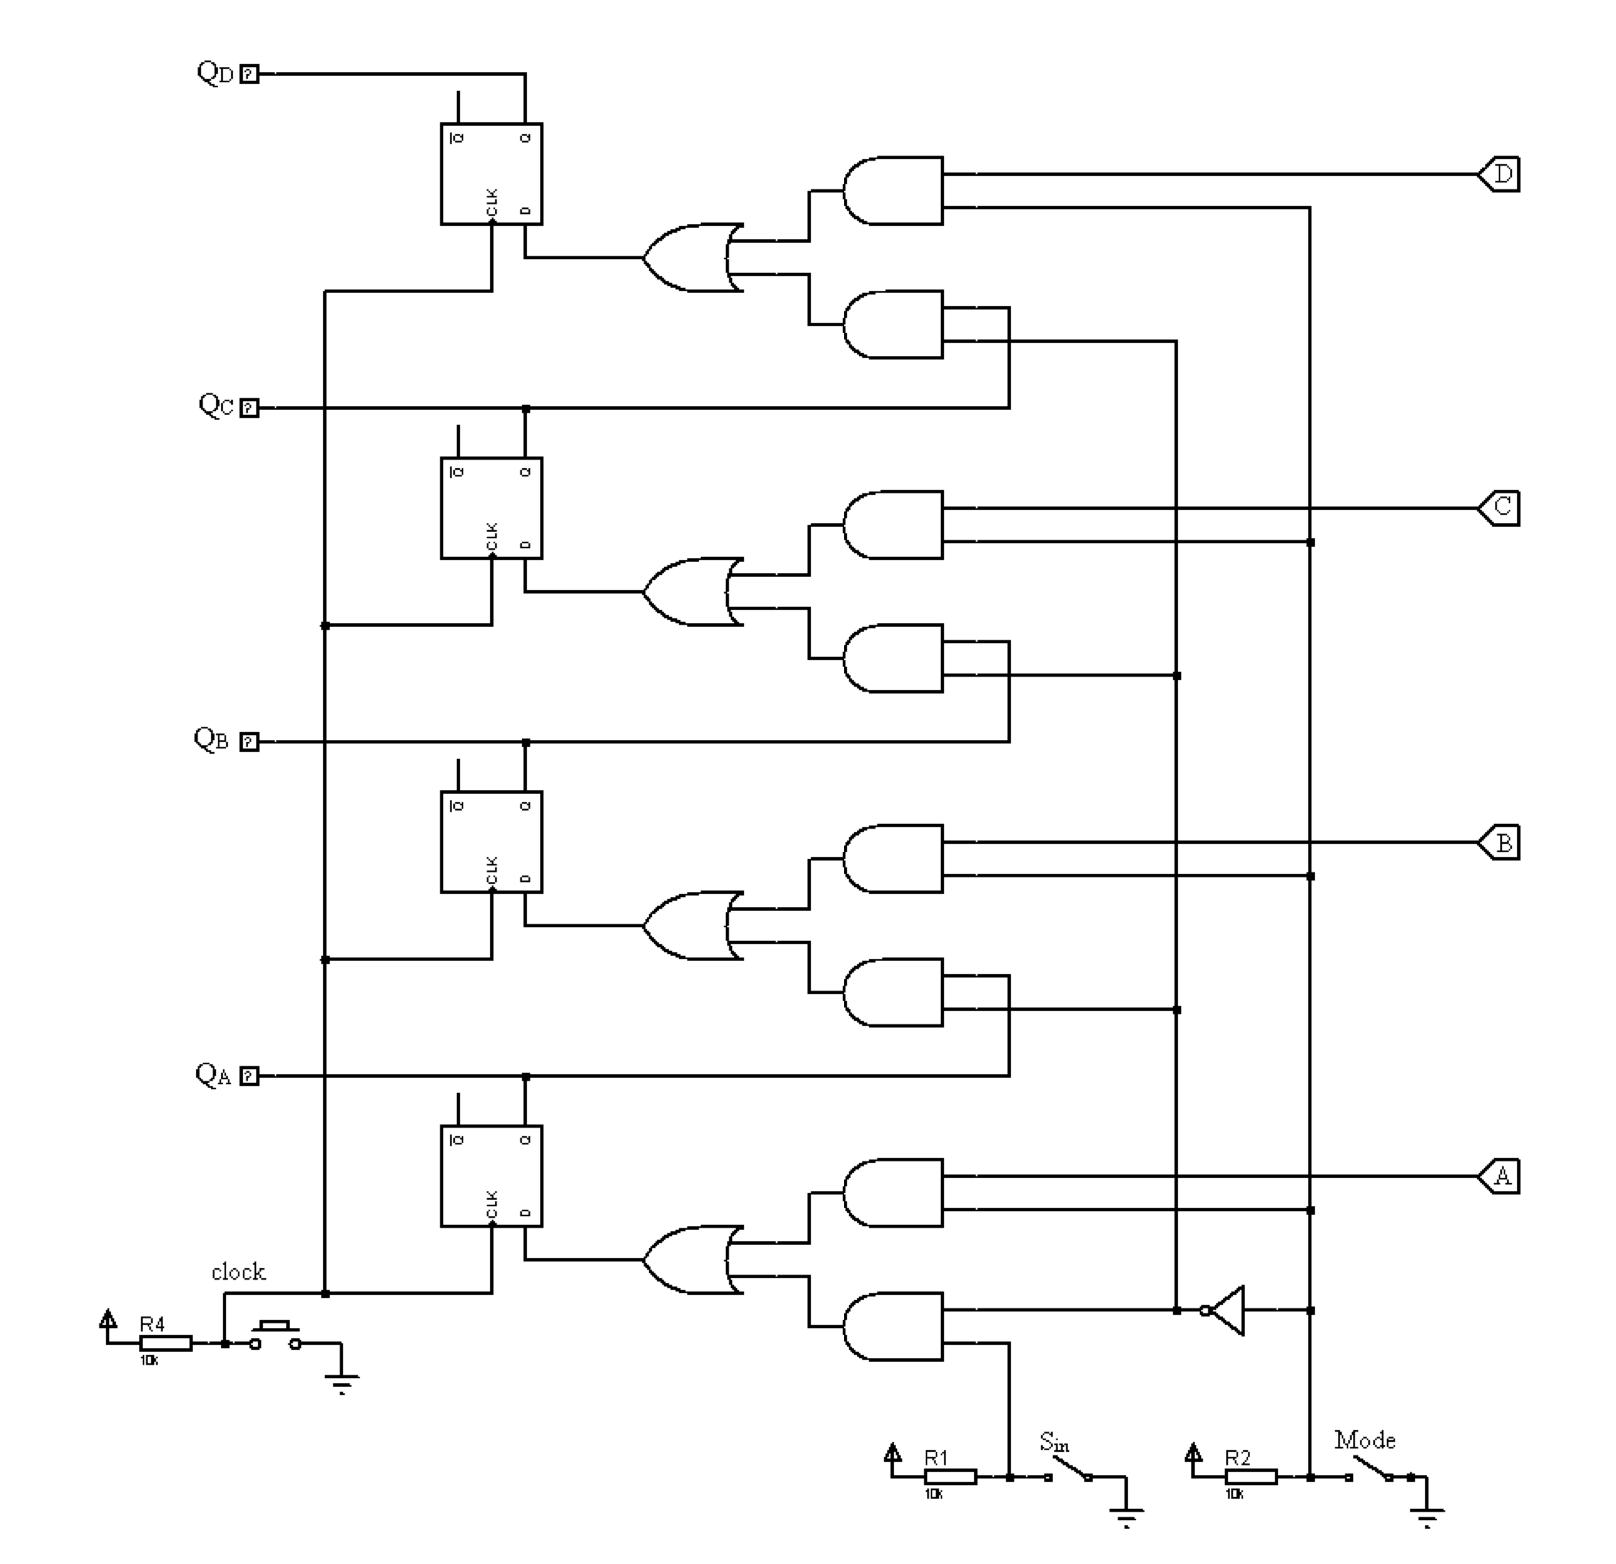
\includegraphics[width=\textwidth]{part1/circuit.png}
    \caption{
    شیفت رجیستر یک طرفه با قابلیت بارگذاری موازی
    }
    \label{fig:circuit1}
\end{figure}

\begin{figure}
    \centering
    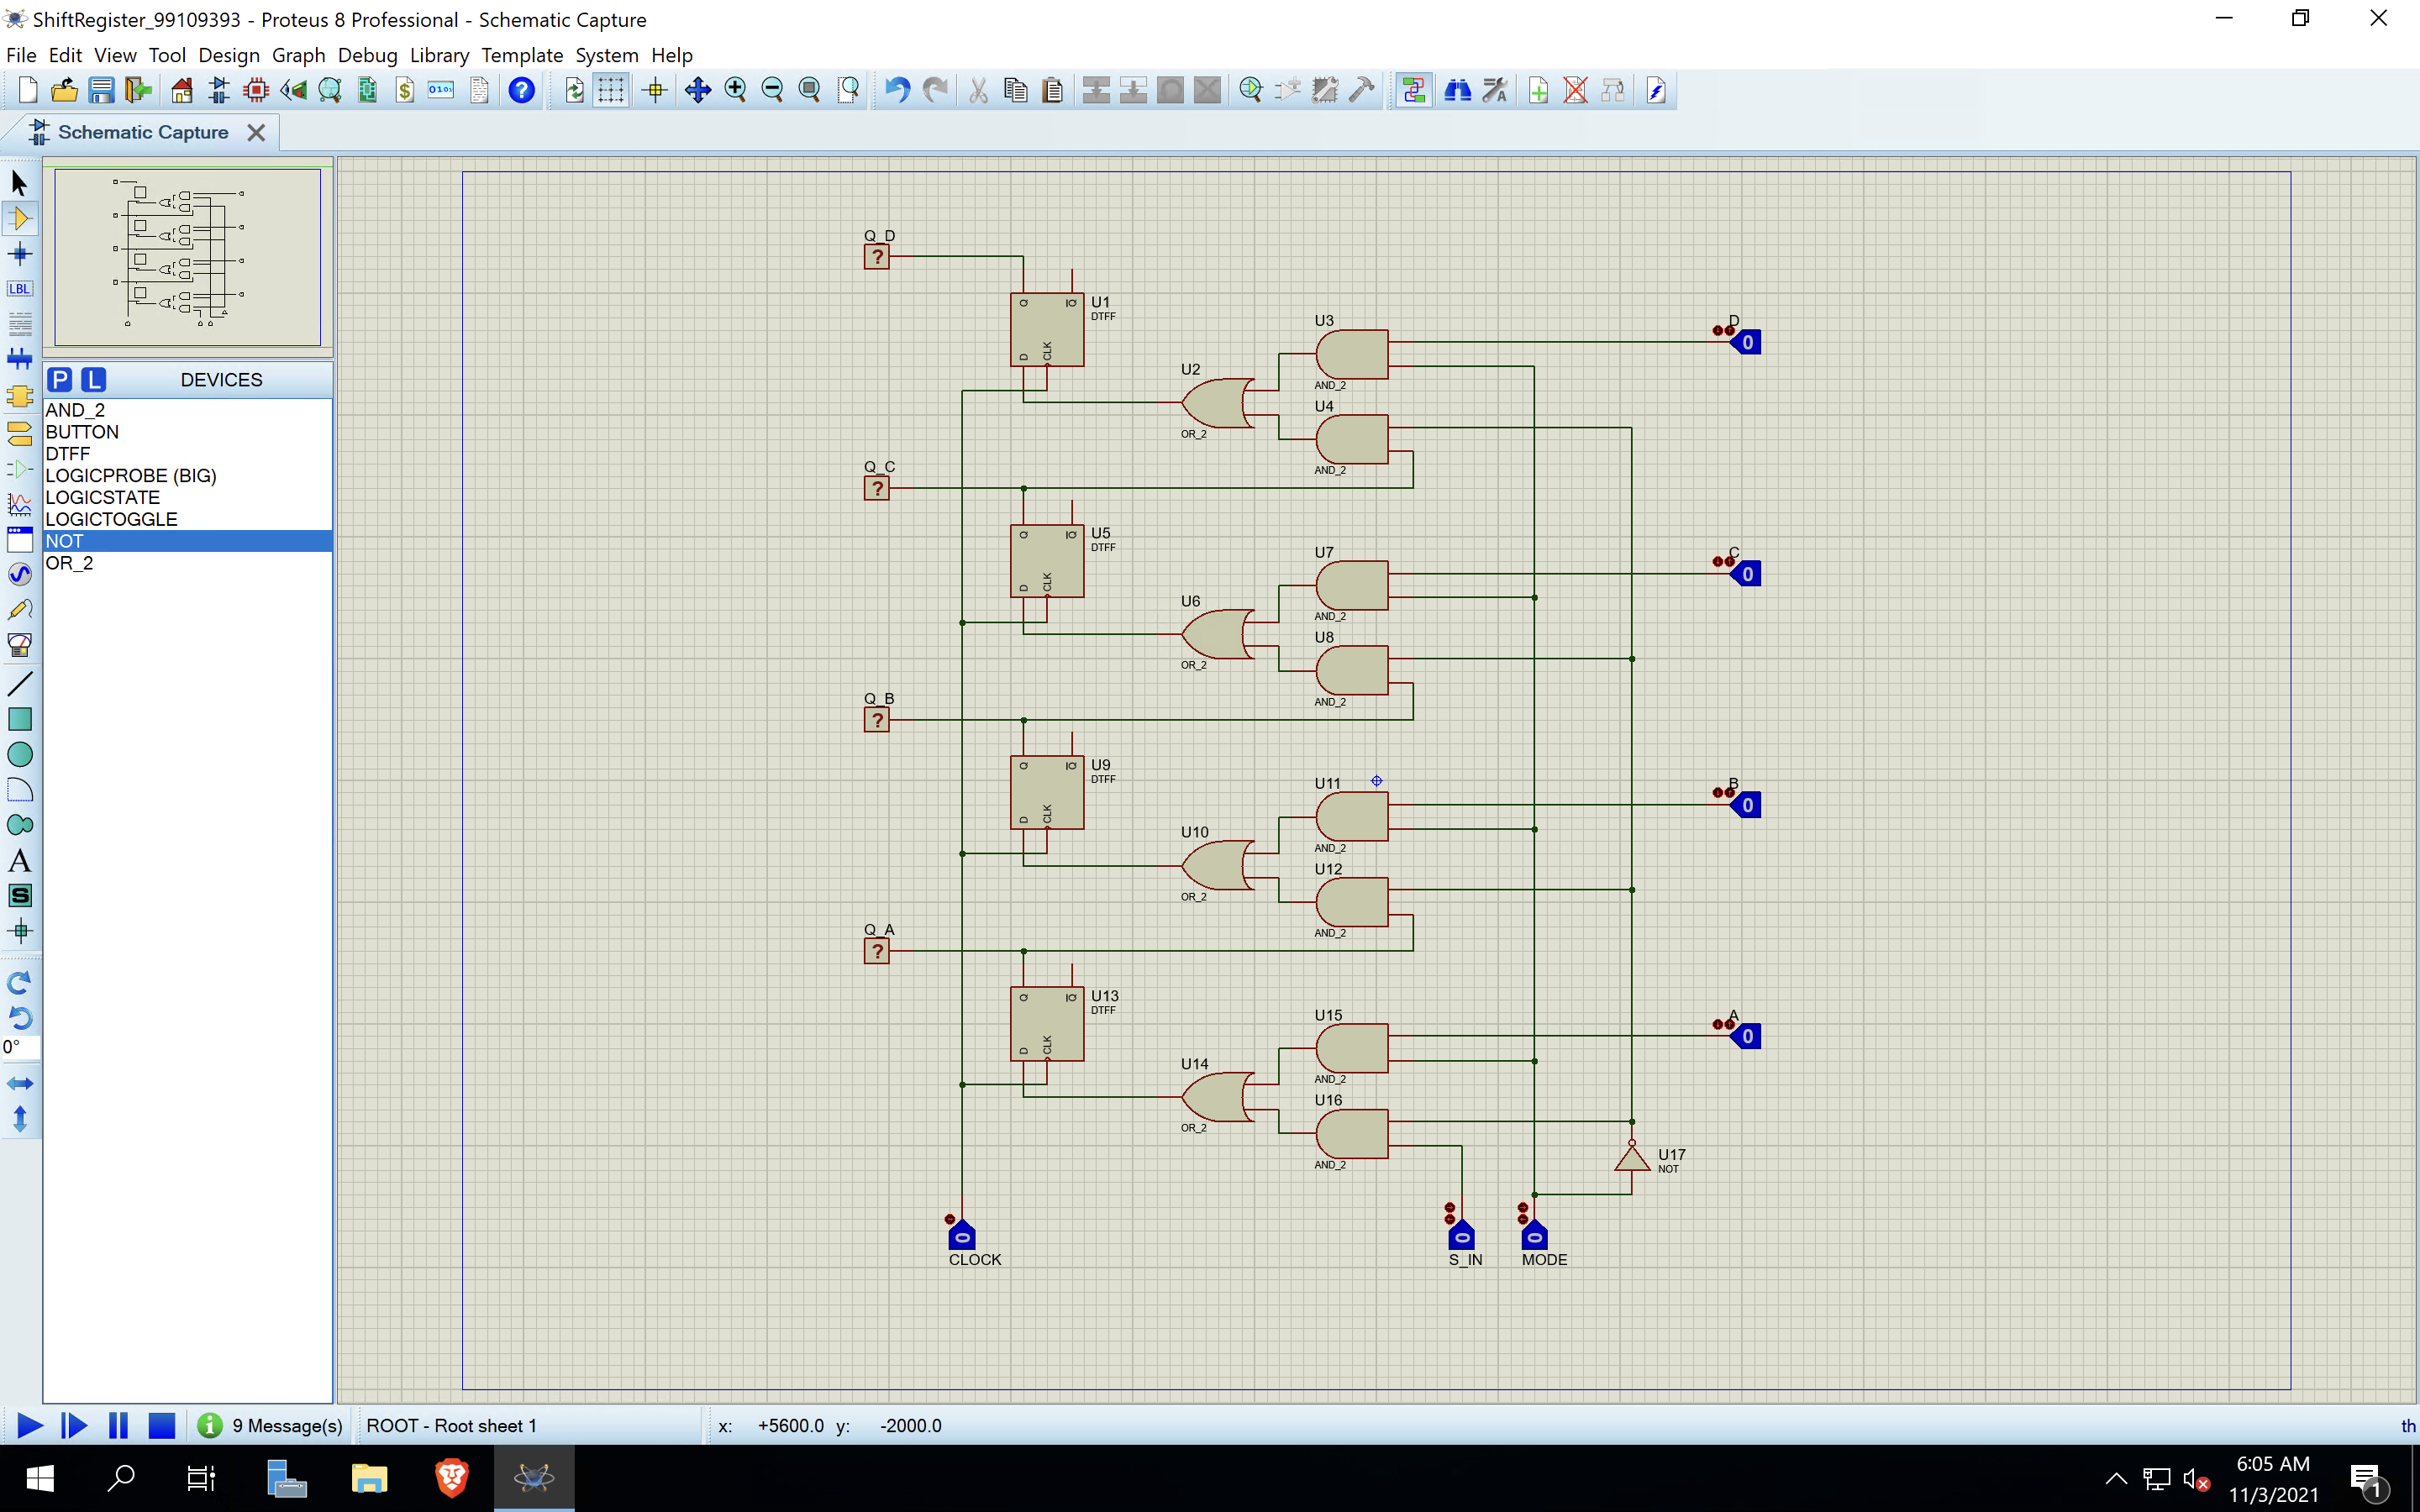
\includegraphics[width=\textwidth]{part1/screen1.png}
    \caption{
    مدار به همراه نام قطعات استفاده شده
    (در سمت چپ)
    }
    \label{fig:circuit2}
\end{figure}

\section{
اعمال یک ورودی
}
در این قسمت با استفاده از قابلیت بازگذاری موازی یا با دادن داده به صورت بیت بیت از بیت ورودی
(بدون استفاده از بارگذاری موازی)
داده را وارد شیفت‌رجیستر می‌کنیم.
در صورت استفاده از بارگذاری موازی تنها یک کلاک لازم است اما در صورت وارد کردن داده از
S\_IN
به چهار کلاک نیاز داریم.
تصویر این کار در شکل
\eqref{fig:circuit3}
آمده است.

\begin{figure}
    \centering
    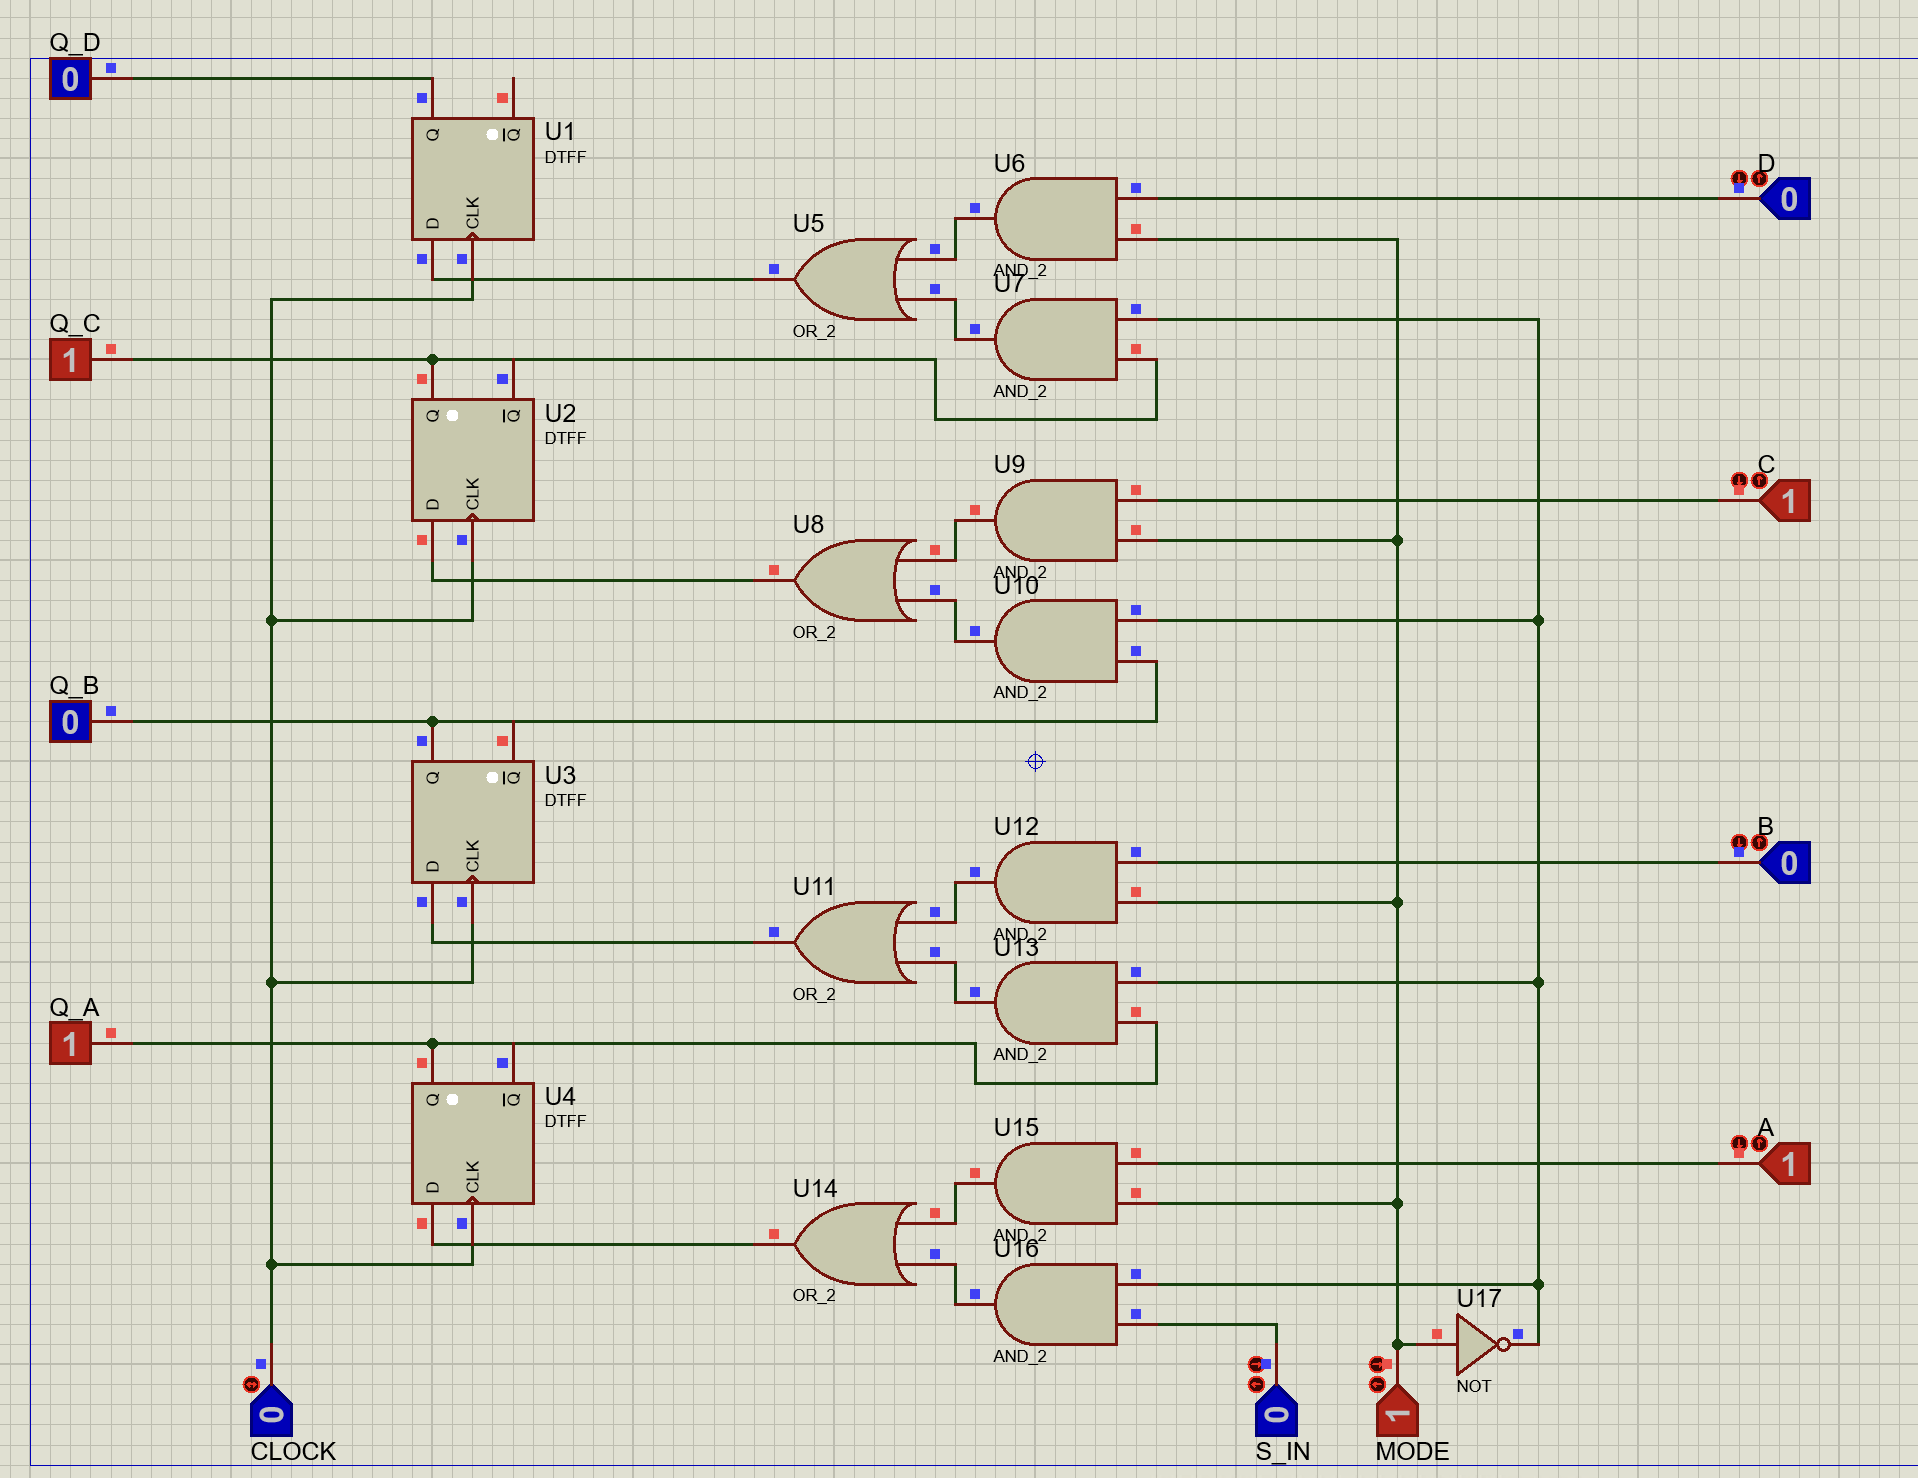
\includegraphics[width=\textwidth]{part1/circuit2.png}
    \caption{
    وارد کردن داده‌ی ۱۰۱۰ با استفاده از بارگذاری موازی
    }
    \label{fig:circuit3}
\end{figure}

\section{
شیفت‌رجیستر با شیف به راست
}
برای این کار کافی است
Mode
را روی ۰ قرار دهیم و
S\_IN
همان ورودی ما خواهد بود.
در صورتی که منظور سوال برعکس کردن جهت فلیپ‌فلاپ
است کافی است به بیت‌های خروجی برعکس نگاه کنیم یا لیبل آن‌ها را برعکس کنیم.
در صورتی که این کار مقدور نبود می‌توانیم جهت گذر اطلاعات بیت‌ها در فلیپ‌فلاپ‌ها را برعکس کنیم یعنی به جای این که بیت خروجی پایینی‌ها به یکی از ورودی‌های
AND
بالایی‌ها برود
برعکس این کار انجام شود و در نهایت هم
S\_IN
به فلیپ‌فلاپ بالا وصل شود.

\section{
شیفت‌رجیستر دوطرفه
}
برای این کار مشابه کاری که بالا توضیح داده شد را انجام می‌دهیم.
به ساختار
MODE
دست نمی‌زنیم و کافی است ورودی‌های مستقیم را حذف کرده و به جای آن‌ها خروجی‌های فلیپ‌فلاپ بالایی هر فلیپ‌فلاپ را قرار دهیم.
انگار که خروجی هر فلیپ‌فلاپ بالایی برای فلیپ‌فلاپ پایینی یک ورودی مستقیم است که در صورت
\lr{MODE = 1}
فعال می‌شود و در غیر این صورت همان شیفت جهت قبل انجام می‌شود.
در نهایت نیز
S\_IN
را به ورودی بارگذاری مستقیم سابق بالاترین فلیپ‌فلاپ هم می‌دهیم چرا که انتظار داریم در حالت شیفت به پایین از این ورودی برای ورودی شیفت‌رجیستر استفاده شود.
(البته می‌توانستیم یک ورودی جدا نیز برای آن در نظر بگیریم تا احتمال خطا در مدار کمتر شود اما ضرورتی ندارد)

تصویر مدار در شکل
\eqref{fig:circuit4}
آمده است.

\begin{figure}
    \centering
    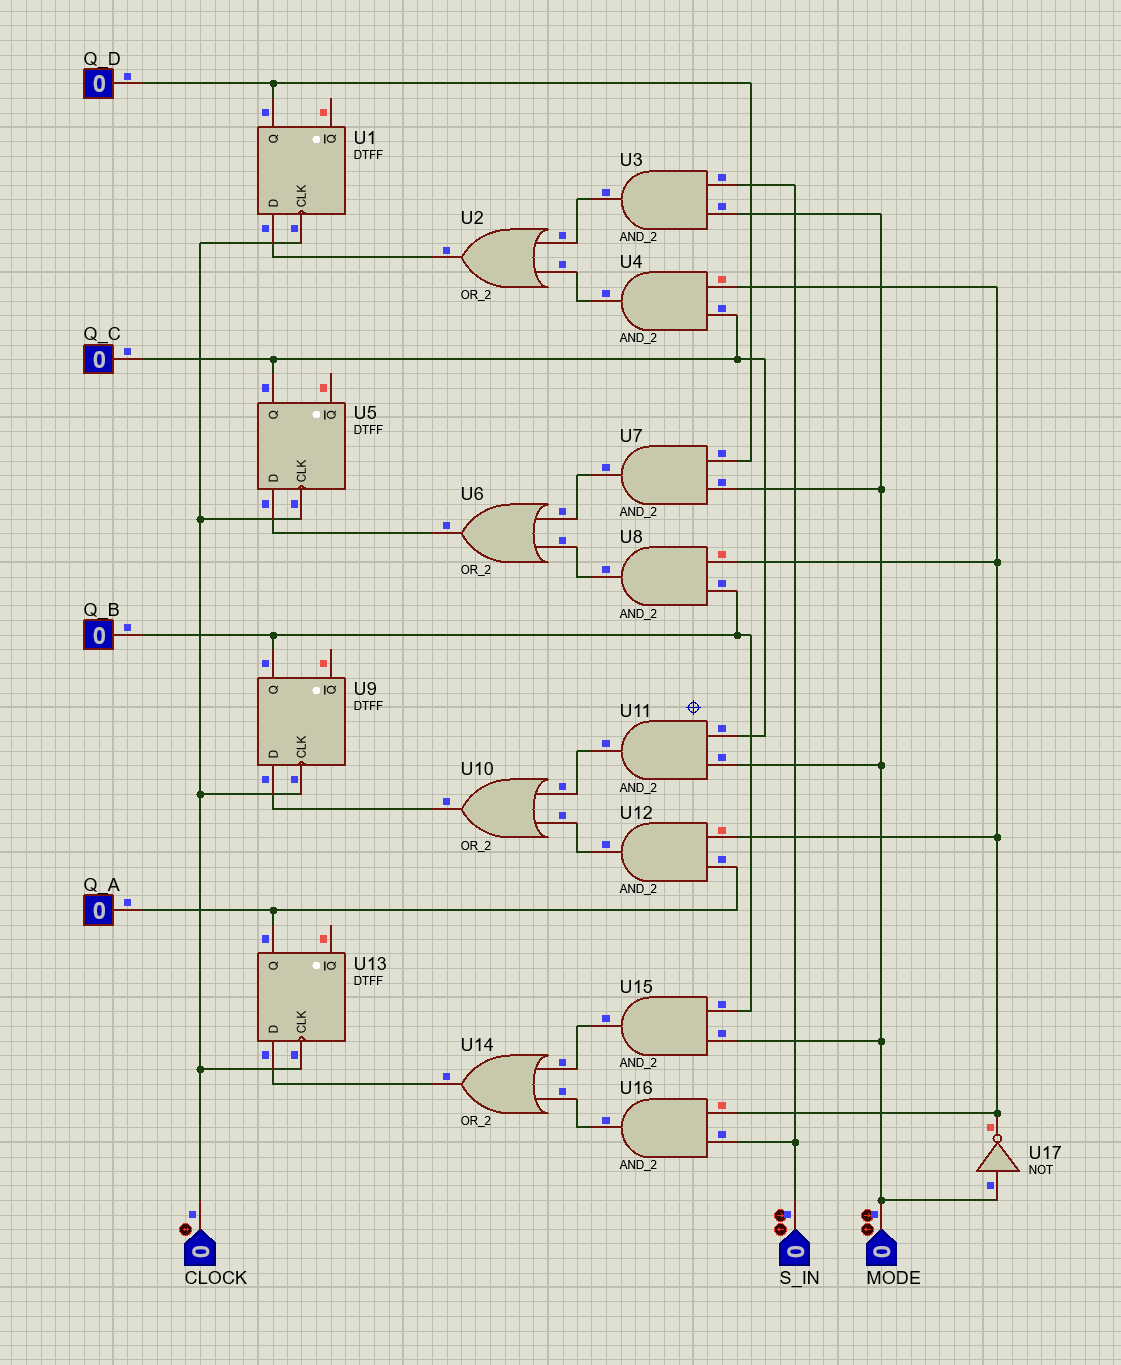
\includegraphics[width=\textwidth]{part1/circuit3.png}
    \caption{
    شیفت‌رجیستر دو طرفه
    }
    \label{fig:circuit4}
\end{figure}